\documentclass[12pt,a4paper]{article}

\usepackage[utf8]{inputenc}
\usepackage[T1]{fontenc}
\usepackage[english]{babel}
\usepackage{graphicx}
\usepackage{float}
\usepackage{geometry}
\usepackage{fancyhdr}
\usepackage{xcolor}
\usepackage{titlesec}
\usepackage{caption}
\usepackage{subcaption}
\usepackage{hyperref}

\geometry{top=2.5cm,bottom=2.5cm,left=3cm,right=3cm}
\graphicspath{{docs/manual-screenshots/}{manual-screenshots/}}

\definecolor{accent}{HTML}{145C4A}
\definecolor{lightgray}{HTML}{E7E9E8}
\definecolor{linkblue}{HTML}{174A66}

\hypersetup{
  colorlinks=true,
  linkcolor=linkblue,
  urlcolor=linkblue,
  pdftitle={KanjiMe --- User Manual},
  pdfauthor={Tycho Quintana Santana}
}

\titleformat{\section}
  {\normalfont\LARGE\bfseries\color{accent}}
  {\thesection}{0.8em}{}
\titleformat{\subsection}
  {\normalfont\Large\bfseries\color{accent}}
  {\thesubsection}{0.7em}{}

\pagestyle{fancy}
\fancyhf{}
\setlength{\headheight}{15pt}
\fancyhead[L]{\nouppercase{\leftmark}}
\fancyfoot[C]{\thepage}
\renewcommand{\headrulewidth}{0.4pt}
\renewcommand{\footrulewidth}{0pt}
\renewcommand{\sectionmark}[1]{\markboth{#1}{}}

\captionsetup{font=small,labelfont=bf}
\setcounter{tocdepth}{2}

\newcommand{\mobilecapture}[3]{%
  \clearpage
  \begin{figure}[H]
    \centering
    \includegraphics[width=0.8\textwidth,height=0.50\textheight,keepaspectratio]{#1}
    \caption{#2}
    \label{#3}
  \end{figure}
}

\newcommand{\desktopcapture}[3]{%
  \clearpage
  \begin{figure}[H]
    \centering
    \includegraphics[width=\textwidth,height=0.45\textheight,keepaspectratio]{#1}
    \caption{#2}
    \label{#3}
  \end{figure}
}

\newcommand{\pendingcapture}[3]{%
  \clearpage
  \begin{figure}[H]
    \centering
    \colorbox{lightgray}{\parbox{0.8\textwidth}{\centering\vspace{2cm}Screenshot pending: \texttt{#1}\vspace{2cm}}}
    \caption{#2}
    \label{#3}
  \end{figure}
}

\begin{document}
\hypersetup{pageanchor=false}

\begin{titlepage}
  \thispagestyle{empty}
  \centering
  \vspace*{2.5cm}
  {\color{accent}\rule{0.82\textwidth}{2pt}\par}
  \vspace{1.4cm}
  {\Huge\bfseries KanjiMe --- User Manual\par}
  \vspace{0.8cm}
  {\LARGE User Manual\par}
  \vspace{1.6cm}
  {\Large Version 1.0.0\par}
  \vspace{0.4cm}
  {\Large June 28, 2026\par}
  \vfill
  \vspace{1.4cm}
  {\color{accent}\rule{0.82\textwidth}{2pt}\par}
\end{titlepage}

\pagenumbering{roman}
\tableofcontents
\clearpage
\listoffigures
\clearpage
\pagenumbering{arabic}
\hypersetup{pageanchor=true}

\newpage
\section{Introduction}

KanjiMe supports kanji study through a mobile application and a separate
administration panel. The mobile application provides character recognition,
search, detailed lookup, calligraphy practice, history, and application
information. The administration panel allows authorised technical-support users
to configure versions and review error reports.

\newpage
\section{Mobile Application}

\subsection{Kanji Recognition}

Recognition identifies kanji from a photograph, a stored image, or strokes
entered on the drawing canvas. Image and Drawing modes share the Results area,
where candidate characters are ordered without numeric confidence values.

Image mode accepts camera input and files from the device. Drawing mode sends
the current canvas strokes for classification. Both paths expose processing and
error states so that the user can distinguish an active operation from a
completed result.

\subsubsection{Initial Image Mode}

Recognition opens in Image mode, as shown in
Figure~\ref{fig:recognition-image-empty}. The empty frame is followed by a
camera button, an image-selection button, and an empty Results area.

\mobilecapture{01-mobile-classification.png}
  {Image mode before a photograph or image has been supplied}
  {fig:recognition-image-empty}

\subsubsection{Camera Input}

Opening the camera displays the inline preview shown in
Figure~\ref{fig:recognition-camera-preview}. A camera control takes the photo,
while the close control returns to the previous Recognition state.

\mobilecapture{40-mobile-classification-camera-preview.png}
  {the inline camera-preview state with capture and close controls}
  {fig:recognition-camera-preview}

If the application cannot take a photo, it displays the centred alert shown in
Figure~\ref{fig:recognition-camera-error}. The alert contains the message ``The
photo could not be captured'' and an OK action.

\mobilecapture{41-mobile-classification-camera-error-alert.png}
  {the controlled camera-capture error alert}
  {fig:recognition-camera-error}

\subsubsection{Uploaded Image and Crop}

After the user selects an image, it appears inside the image frame. The helper
text explains that dragging over the image refines the area to classify.

The Results section in Figure~\ref{fig:recognition-image-results} lists the
predicted characters in order. Each row includes the character and its
associated reading or level information.

\mobilecapture{44-mobile-classification-image-results.png}
  {image-classification results below the uploaded source}
  {fig:recognition-image-results}

Dragging over the source creates the highlighted rectangular crop shown in
Figure~\ref{fig:recognition-image-crop}. The area outside the selection is
shaded.

\mobilecapture{45-mobile-classification-image-crop-overlay.png}
  {the crop overlay over an uploaded image}
  {fig:recognition-image-crop}

\subsubsection{Drawing Input}

Selecting Drawing replaces the image controls with the empty square canvas in
Figure~\ref{fig:recognition-drawing-empty}. A paper-bin control appears below
the canvas and Results remains underneath.

\mobilecapture{02-mobile-classification-drawing.png}
  {Drawing mode with an empty canvas}
  {fig:recognition-drawing-empty}

While the application processes the drawing, the progress indicator shown in
Figure~\ref{fig:recognition-drawing-processing} appears beside the Results
heading.

\mobilecapture{47-mobile-classification-drawing-processing.png}
  {drawing classification while a stroke is being processed}
  {fig:recognition-drawing-processing}

When processing finishes, the ranked list in
Figure~\ref{fig:recognition-drawing-results} appears beneath the drawing. Its
rows show characters, readings, and levels without numeric confidence values.

\mobilecapture{48-mobile-classification-drawing-results.png}
  {drawing-classification results after strokes were entered}
  {fig:recognition-drawing-results}

\subsubsection{Recognition Loading}

The model-loading overlay in Figure~\ref{fig:recognition-model-loading} informs
the user that character recognition is being prepared.

\mobilecapture{18-mobile-model-loading.png}
  {Recognition-model loading overlay}
  {fig:recognition-model-loading}

\newpage
\subsection{Kanji Search and Lookup}

Search accepts a kanji or reading and returns matching entries from the local
data set. Each result combines the character with its principal readings and
classification levels when those values are available.

Selecting a result opens its reference entry. The detail view separates
meanings, readings, structural information, examples, and stroke order so that
each category can be reviewed independently.

\subsubsection{Search States}

The Search screen in Figure~\ref{fig:search-empty} has a ``Kanji or reading''
field and a Results panel. Before a query is entered, the panel states that no
matching kanji were found.

\mobilecapture{03-mobile-search-empty.png}
  {the Search screen before a query is entered}
  {fig:search-empty}

While a search is in progress, the query remains in the field and the Results
panel is temporarily blank, as shown in Figure~\ref{fig:search-searching}.

\mobilecapture{51-mobile-search-searching.png}
  {the intermediate search state before results are displayed}
  {fig:search-searching}

A query with no matches retains the entered text and displays the no-results
message shown in Figure~\ref{fig:search-no-results}.

\mobilecapture{52-mobile-search-no-results.png}
  {a completed search with no matching result}
  {fig:search-no-results}

A successful search displays the result rows shown in
Figure~\ref{fig:search-results}. Each row combines a character, its readings,
and any available JLPT or Joyo information.

\mobilecapture{04-mobile-search-results-day.png}
  {search results for the captured day/sun character query}
  {fig:search-results}

\subsubsection{Character Lookup}

The successful detail screen in Figure~\ref{fig:lookup-detail} displays the
character at the top, followed by Meaning, Readings, Information, and Examples.
Reference fields include radical, components, stroke count, and JLPT/Joyo
level. Back and copy controls appear in the header.

\mobilecapture{05-mobile-kanji-day-detail.png}
  {the upper portion of a populated kanji detail screen}
  {fig:lookup-detail}

Farther down the same detail view, the Stroke order section in
Figure~\ref{fig:lookup-stroke-order} displays a drawn stroke-order graphic.

\mobilecapture{55-mobile-kanji-stroke-order.png}
  {the lower detail view containing examples and stroke order}
  {fig:lookup-stroke-order}

An invalid lookup produces the error state shown in
Figure~\ref{fig:lookup-error}. Red text states that the character details could
not be loaded.

\mobilecapture{54-mobile-kanji-error.png}
  {the kanji detail error state}
  {fig:lookup-error}

\newpage
\subsection{Calligraphy Practice}

Calligraphy Practice organises characters by JLPT level or Joyo grade before a
practice session begins. Each category displays its number of available kanji,
which defines the set presented in the selection view.

After selecting a character, the user reproduces it on a dedicated canvas and
submits the attempt for evaluation. The result compares the attempt with the
reference form using stroke and shape metrics.

\subsubsection{Category Groups}

The Calligraphy home screen in Figure~\ref{fig:calligraphy-jlpt-categories} has
JLPT and Joyo selectors. With JLPT active, the visible categories are N5 through
N1 and Unclassified, each accompanied by a kanji count.

\mobilecapture{06-mobile-calligraphy-home.png}
  {the Calligraphy home screen with JLPT categories}
  {fig:calligraphy-jlpt-categories}

The Joyo variant in Figure~\ref{fig:calligraphy-joyo-categories} lists
grade-based categories and their visible counts.

\mobilecapture{56-mobile-calligraphy-joyo.png}
  {the Calligraphy home screen with Joyo grade categories}
  {fig:calligraphy-joyo-categories}

\subsubsection{Character Selection}

Opening a JLPT category presents the search field and scrollable character list
shown in Figure~\ref{fig:calligraphy-category}. Each row includes a stroke
count.

\mobilecapture{07-mobile-calligraphy-jlpt-n5.png}
  {the character list for the captured JLPT N5 route}
  {fig:calligraphy-category}

The filter narrows the list and preserves each character's stroke count, as
shown in Figure~\ref{fig:calligraphy-category-filtered}.

\mobilecapture{57-mobile-calligraphy-category-filtered.png}
  {a filtered calligraphy category list}
  {fig:calligraphy-category-filtered}

When the filter has no matches, the list area displays ``No kanji are available
in this category'', as shown in Figure~\ref{fig:calligraphy-category-empty}.

\mobilecapture{58-mobile-calligraphy-category-empty.png}
  {the empty result state within a calligraphy category}
  {fig:calligraphy-category-empty}

\subsubsection{Practice and Evaluation}

The initial practice view in Figure~\ref{fig:calligraphy-practice-empty} has a
large empty canvas. Back, delete, and validation controls appear in the top row.
Delete and validation remain inactive until the user draws on the canvas.

\mobilecapture{08-mobile-calligraphy-practice-day.png}
  {the calligraphy practice canvas before drawing}
  {fig:calligraphy-practice-empty}

As the user draws, the strokes appear on the canvas, as shown in
Figure~\ref{fig:calligraphy-practice-drawing}. The delete and validation
controls remain available in the toolbar.

\mobilecapture{59-mobile-calligraphy-practice-drawing.png}
  {the calligraphy practice canvas with visible strokes}
  {fig:calligraphy-practice-drawing}

The evaluation overlay in Figure~\ref{fig:calligraphy-evaluation} shows the
score and a short summary. It compares separate Reference and Attempt images and
reports metrics for stroke count, stroke order, direction, and similarity.

\mobilecapture{60-mobile-calligraphy-evaluation.png}
  {the calligraphy evaluation overlay for the captured attempt}
  {fig:calligraphy-evaluation}

\newpage
\subsection{History}

History separates recent activity into four icon-based categories. The
categories cover searches, visited entries, image classifications, and drawing
classifications.

Each populated row identifies the recorded kanji and retains the information
needed to recognise the activity. The search tab in
Figure~\ref{fig:history-search} includes the character, readings, and date.

\mobilecapture{09-mobile-history.png}
  {History with one recorded search entry}
  {fig:history-search}

When the selected category has no entries, the four category controls remain
available and the list stays empty, as shown in Figure~\ref{fig:history-empty}.

\mobilecapture{62-mobile-history-empty.png}
  {History with no visible entries in the selected category}
  {fig:history-empty}

The remaining tabs organise visited kanji, image classifications, and drawing
classifications into separate history views. These views appear in
Figures~\ref{fig:history-visited}, \ref{fig:history-image-classifications}, and
\ref{fig:history-drawing-classifications}.

\begin{figure}[H]
  \centering
  \begin{subfigure}[t]{0.31\textwidth}
    \centering
    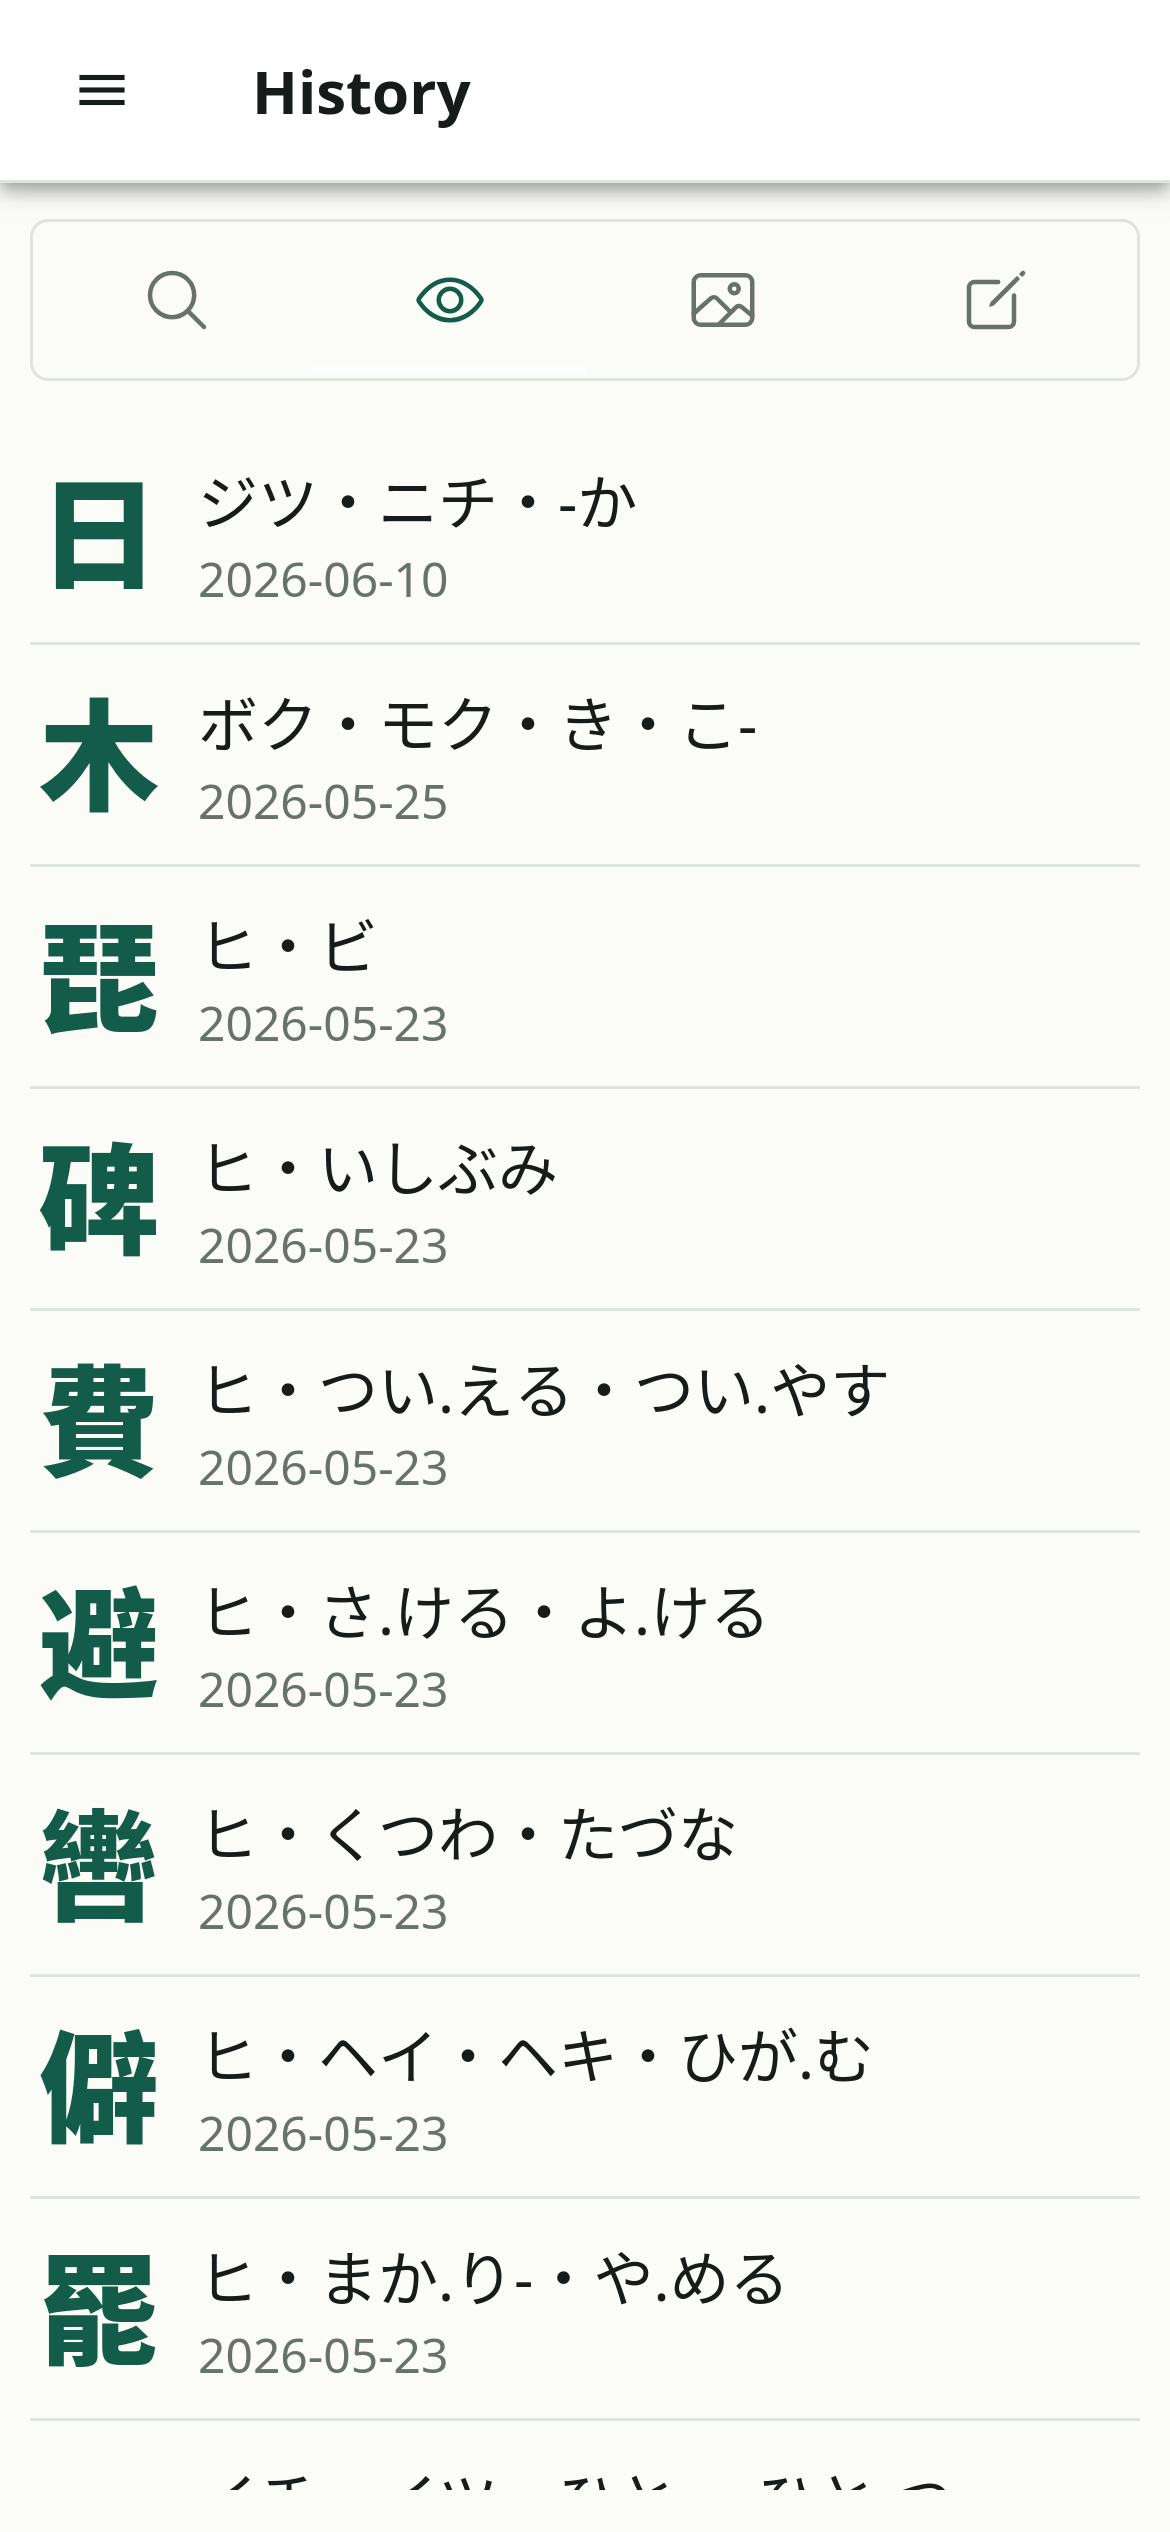
\includegraphics[width=\textwidth,height=0.42\textheight,keepaspectratio]{63-mobile-history-visited.png}
    \caption{History view for visited kanji}
    \label{fig:history-visited}
  \end{subfigure}
  \hfill
  \begin{subfigure}[t]{0.31\textwidth}
    \centering
    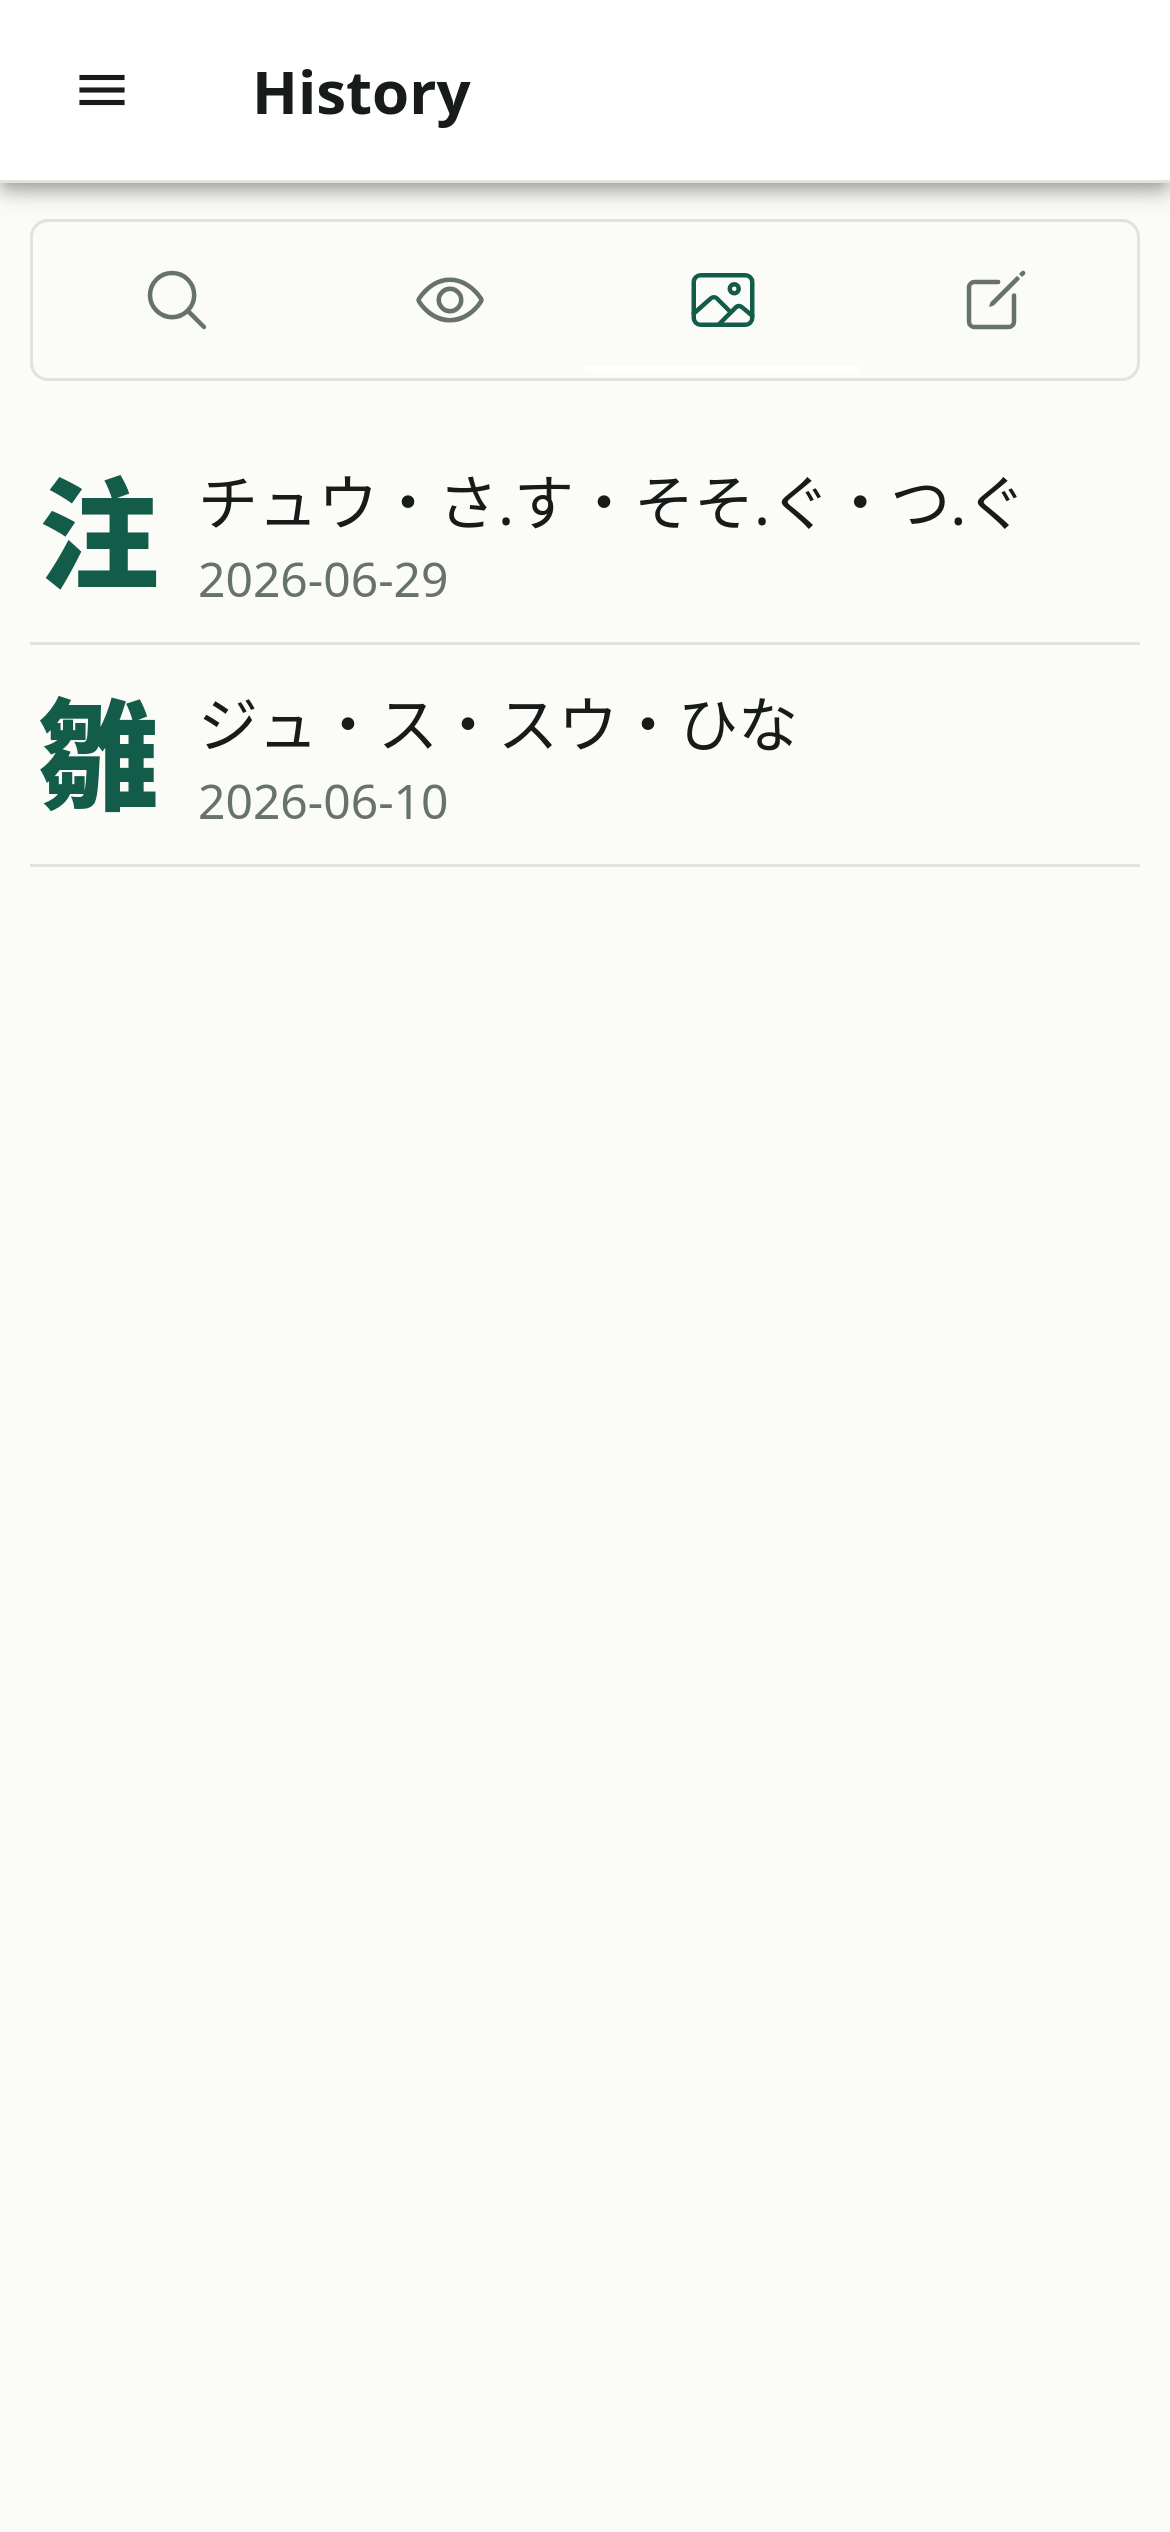
\includegraphics[width=\textwidth,height=0.42\textheight,keepaspectratio]{64-mobile-history-image-classification.png}
    \caption{History view for image classifications}
    \label{fig:history-image-classifications}
  \end{subfigure}
  \hfill
  \begin{subfigure}[t]{0.31\textwidth}
    \centering
    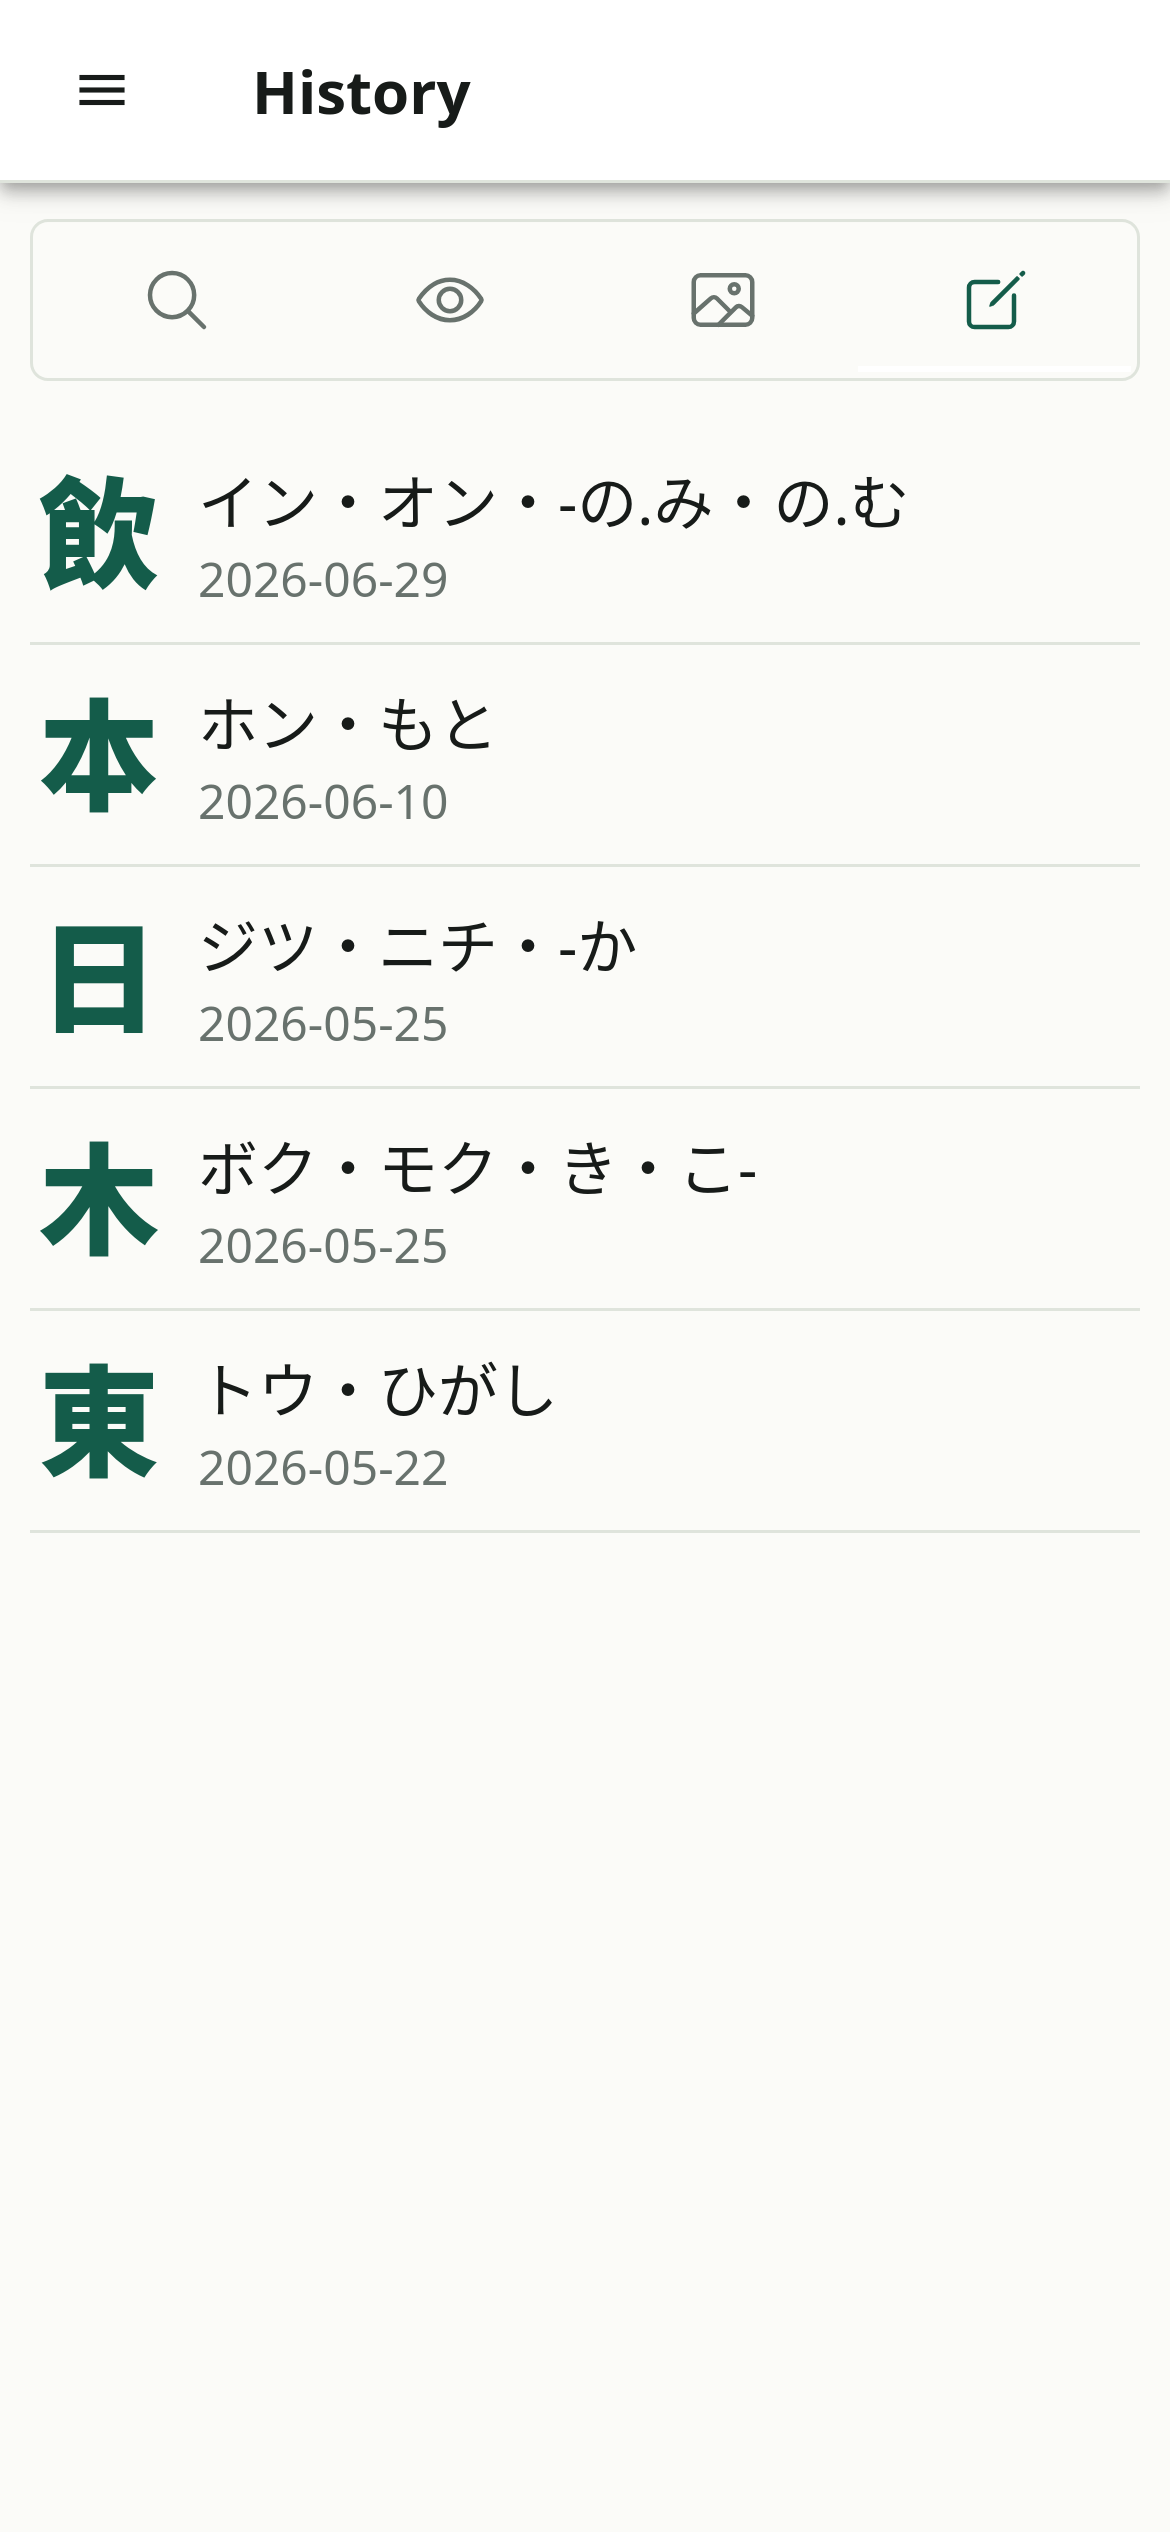
\includegraphics[width=\textwidth,height=0.42\textheight,keepaspectratio]{65-mobile-history-drawing-classification.png}
    \caption{History view for drawing classifications}
    \label{fig:history-drawing-classifications}
  \end{subfigure}
\end{figure}

\newpage
\subsection{App Information}

The About view identifies the installed KanjiMe version and records the
application's authorship. It also contains the notices required for the language
and character data included with the mobile application.

The source acknowledgements name JMdict, KANJIDIC2, KanjiVG, ETL9B, and the
Tanos JLPT kanji lists. Figure~\ref{fig:about-information} presents the version,
authorship, and first part of these notices. The continuation in
Figure~\ref{fig:about-acknowledgements} contains the remaining acknowledgements
and licence text.

\begin{figure}[H]
  \centering
  \begin{subfigure}[t]{0.47\textwidth}
    \centering
    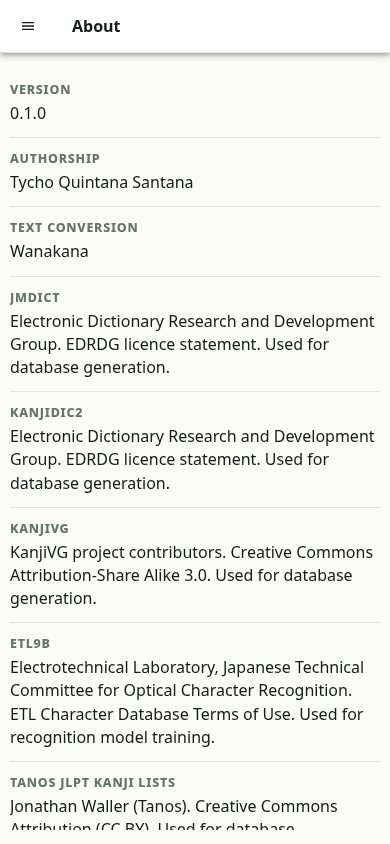
\includegraphics[width=\textwidth,height=0.48\textheight,keepaspectratio]{10-mobile-about.png}
    \caption{the upper portion of the About information}
    \label{fig:about-information}
  \end{subfigure}
  \hfill
  \begin{subfigure}[t]{0.47\textwidth}
    \centering
    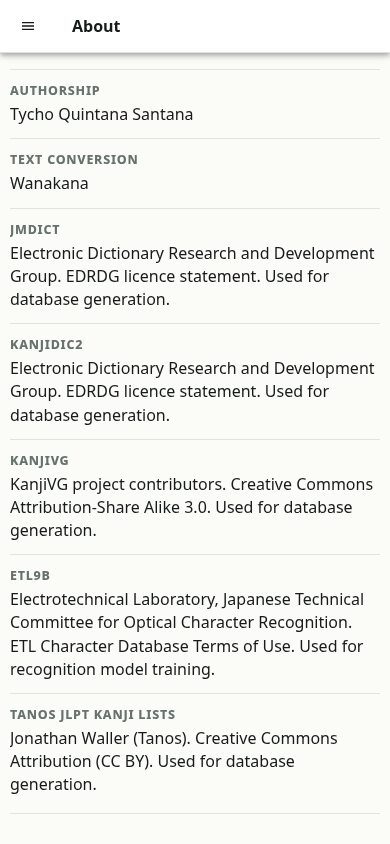
\includegraphics[width=\textwidth,height=0.48\textheight,keepaspectratio]{67-mobile-about-bottom.png}
    \caption{the lower portion of the About acknowledgements}
    \label{fig:about-acknowledgements}
  \end{subfigure}
\end{figure}

\newpage
\subsection{Theme and Language}

The side menu provides access to Recognition, Search, History, Calligraphy, and
About. Theme and language controls appear in the same navigation panel, keeping
display preferences separate from study functions.

The selected theme applies to backgrounds, surfaces, borders, text, and accent
colours throughout the mobile views. Figure~\ref{fig:theme-light-menu} presents
the complete menu in the light theme. Figure~\ref{fig:navigation-menu-opening}
records the same panel while it opens over Recognition.

\begin{figure}[H]
  \centering
  \begin{subfigure}[t]{0.47\textwidth}
    \centering
    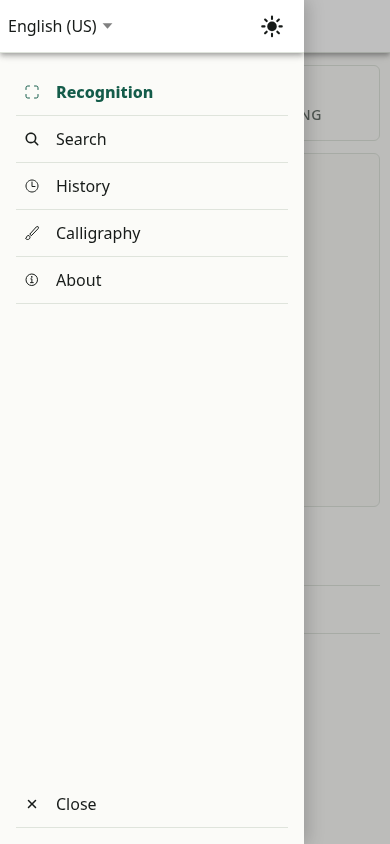
\includegraphics[width=\textwidth,height=0.48\textheight,keepaspectratio]{20-mobile-theme-light-menu.png}
    \caption{the navigation menu in the explicit light theme}
    \label{fig:theme-light-menu}
  \end{subfigure}
  \hfill
  \begin{subfigure}[t]{0.47\textwidth}
    \centering
    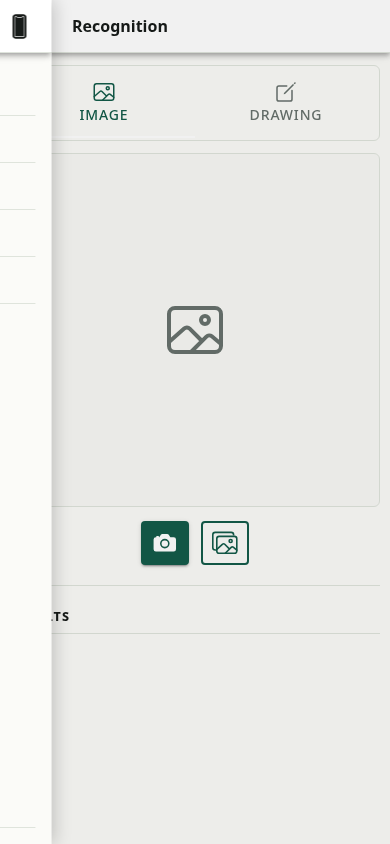
\includegraphics[width=\textwidth,height=0.48\textheight,keepaspectratio]{11-mobile-side-menu.png}
    \caption{a partially visible side-menu state over the Recognition screen}
    \label{fig:navigation-menu-opening}
  \end{subfigure}
\end{figure}

Changing the theme updates the application background, surfaces, borders, text,
and accent colours without changing the Recognition controls. The dark
Recognition screen in Figure~\ref{fig:theme-dark-recognition} retains the Image
and Drawing choices, and the corresponding menu in
Figure~\ref{fig:theme-dark-menu}
retains the same destinations as its light counterpart.

\begin{figure}[H]
  \centering
  \begin{subfigure}[t]{0.47\textwidth}
    \centering
    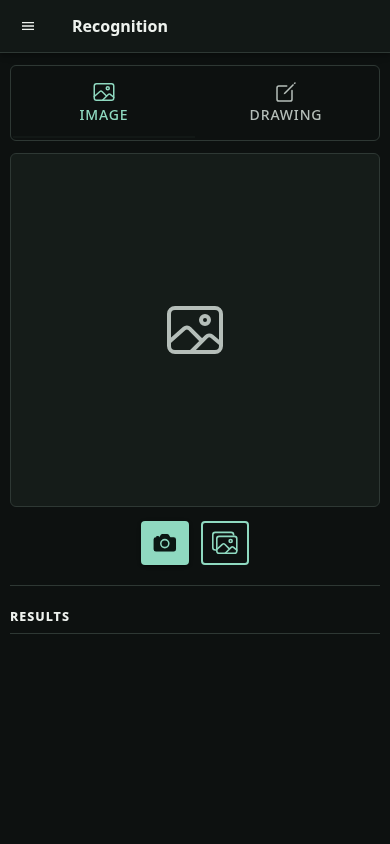
\includegraphics[width=\textwidth,height=0.48\textheight,keepaspectratio]{21-mobile-theme-dark-classification.png}
    \caption{the Recognition screen in the dark theme}
    \label{fig:theme-dark-recognition}
  \end{subfigure}
  \hfill
  \begin{subfigure}[t]{0.47\textwidth}
    \centering
    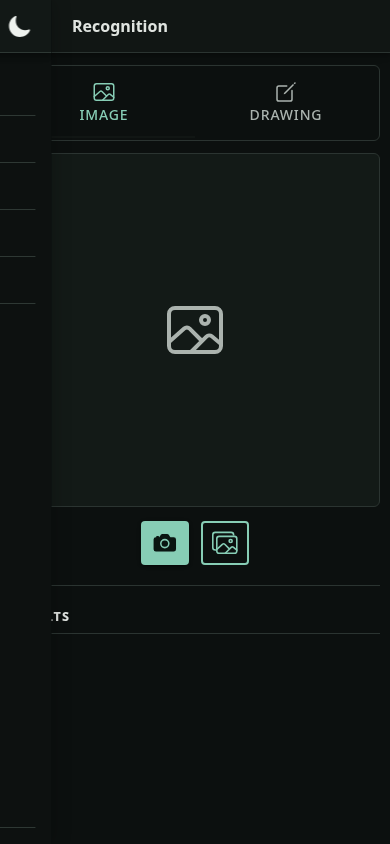
\includegraphics[width=\textwidth,height=0.48\textheight,keepaspectratio]{22-mobile-theme-dark-menu.png}
    \caption{the navigation menu in the dark theme}
    \label{fig:theme-dark-menu}
  \end{subfigure}
\end{figure}

The language control opens the selection sheet shown in
Figure~\ref{fig:language-selector}. The available choices visible there include
English variants and languages from Europe, Asia, and Africa, with a Cancel
action for closing the sheet without selecting another language.

\mobilecapture{19-mobile-language-selector.png}
  {the open language-selection sheet}
  {fig:language-selector}

The available European language selections appear in
Figures~\ref{fig:locale-en-gb}, \ref{fig:locale-es-es}, \ref{fig:locale-fr-fr},
\ref{fig:locale-de-de}, \ref{fig:locale-it-it}, and
\ref{fig:locale-pt-pt}. Asian language selections appear in
Figures~\ref{fig:locale-ja-jp}, \ref{fig:locale-zh-cn},
\ref{fig:locale-zh-tw}, \ref{fig:locale-ko-kr}, and
\ref{fig:locale-hi-in}. Figures~\ref{fig:locale-ar-sa},
\ref{fig:locale-sw-ke}, \ref{fig:locale-am-et}, \ref{fig:locale-ha-ng},
\ref{fig:locale-yo-ng}, and \ref{fig:locale-zu-za} show the remaining
selections. Depending on the open view, translated text appears in the
navigation menu or on the Recognition screen.

\begin{figure}[H]
  \centering
  \begin{subfigure}[t]{0.31\textwidth}
    \centering
    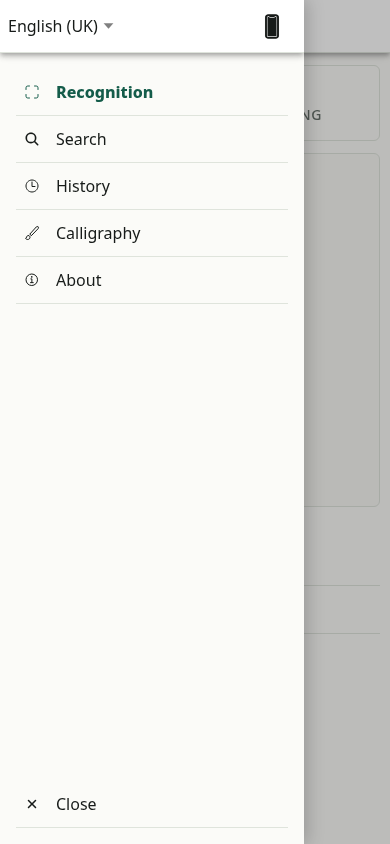
\includegraphics[width=\textwidth,height=0.36\textheight,keepaspectratio]{23-mobile-locale-en-gb.png}
    \caption{the mobile interface with English (UK) selected}
    \label{fig:locale-en-gb}
  \end{subfigure}
  \hfill
  \begin{subfigure}[t]{0.31\textwidth}
    \centering
    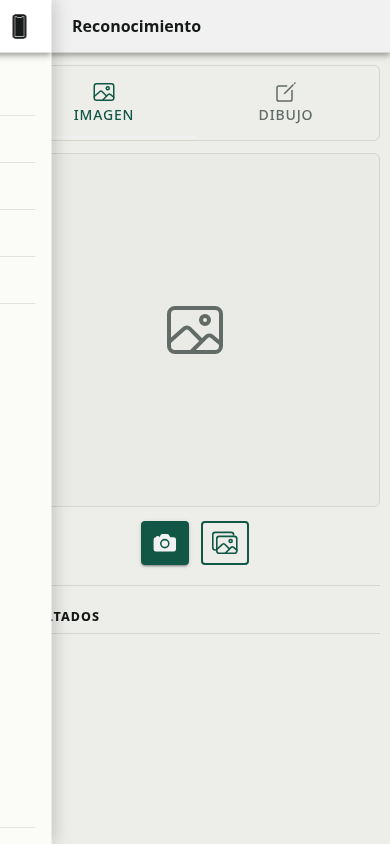
\includegraphics[width=\textwidth,height=0.36\textheight,keepaspectratio]{24-mobile-locale-es-es.png}
    \caption{the mobile interface with Spanish selected}
    \label{fig:locale-es-es}
  \end{subfigure}
  \hfill
  \begin{subfigure}[t]{0.31\textwidth}
    \centering
    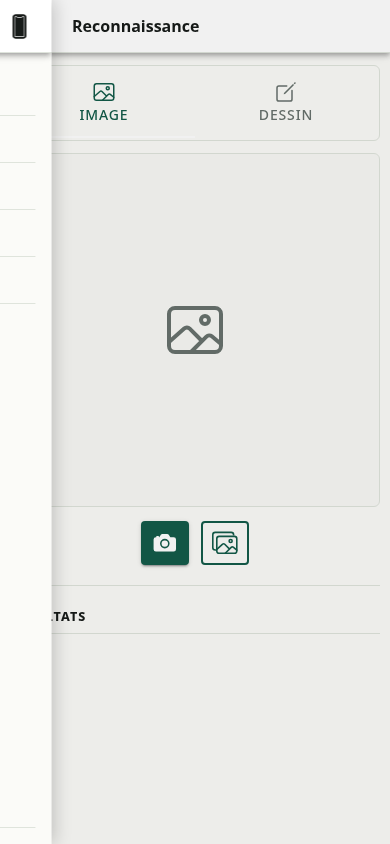
\includegraphics[width=\textwidth,height=0.36\textheight,keepaspectratio]{25-mobile-locale-fr-fr.png}
    \caption{the mobile interface with French selected}
    \label{fig:locale-fr-fr}
  \end{subfigure}
\end{figure}

\begin{figure}[H]
  \centering
  \begin{subfigure}[t]{0.31\textwidth}
    \centering
    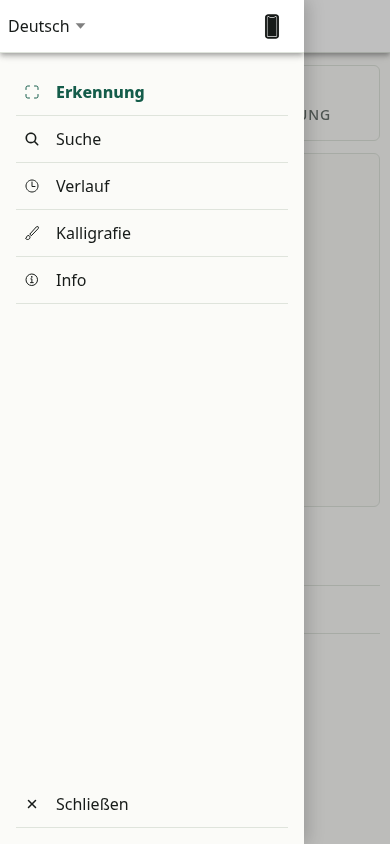
\includegraphics[width=\textwidth,height=0.36\textheight,keepaspectratio]{26-mobile-locale-de-de.png}
    \caption{the mobile interface with German selected}
    \label{fig:locale-de-de}
  \end{subfigure}
  \hfill
  \begin{subfigure}[t]{0.31\textwidth}
    \centering
    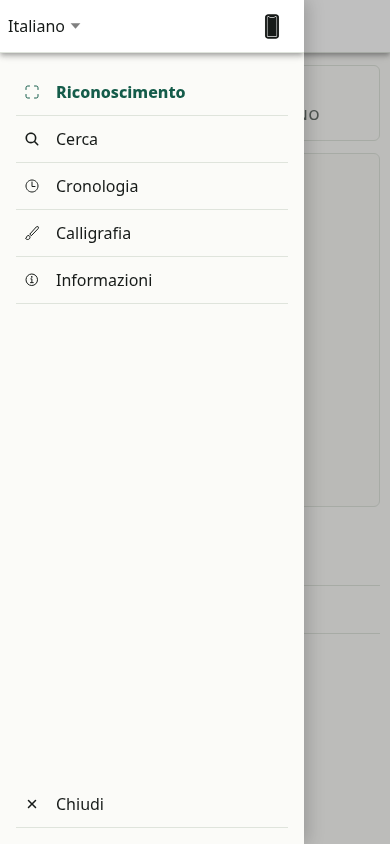
\includegraphics[width=\textwidth,height=0.36\textheight,keepaspectratio]{27-mobile-locale-it-it.png}
    \caption{the mobile interface with Italian selected}
    \label{fig:locale-it-it}
  \end{subfigure}
  \hfill
  \begin{subfigure}[t]{0.31\textwidth}
    \centering
    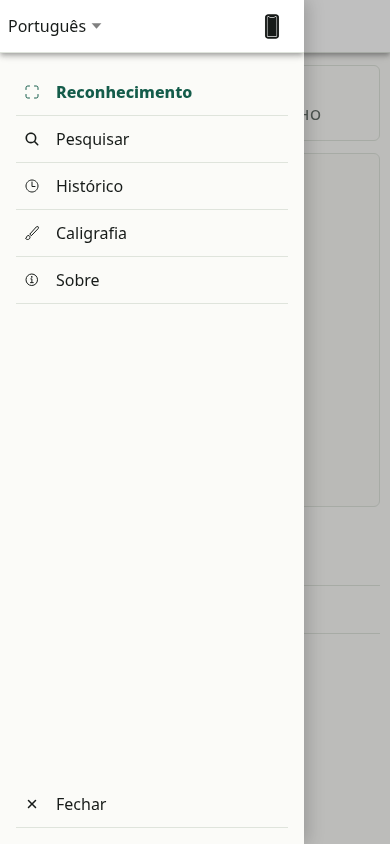
\includegraphics[width=\textwidth,height=0.36\textheight,keepaspectratio]{28-mobile-locale-pt-pt.png}
    \caption{the mobile interface with Portuguese selected}
    \label{fig:locale-pt-pt}
  \end{subfigure}
\end{figure}

\begin{figure}[H]
  \centering
  \begin{subfigure}[t]{0.31\textwidth}
    \centering
    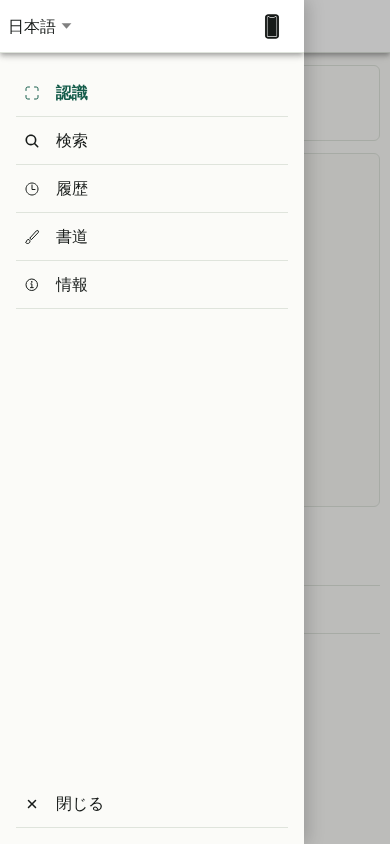
\includegraphics[width=\textwidth,height=0.36\textheight,keepaspectratio]{29-mobile-locale-ja-jp.png}
    \caption{the mobile interface with Japanese selected}
    \label{fig:locale-ja-jp}
  \end{subfigure}
  \hfill
  \begin{subfigure}[t]{0.31\textwidth}
    \centering
    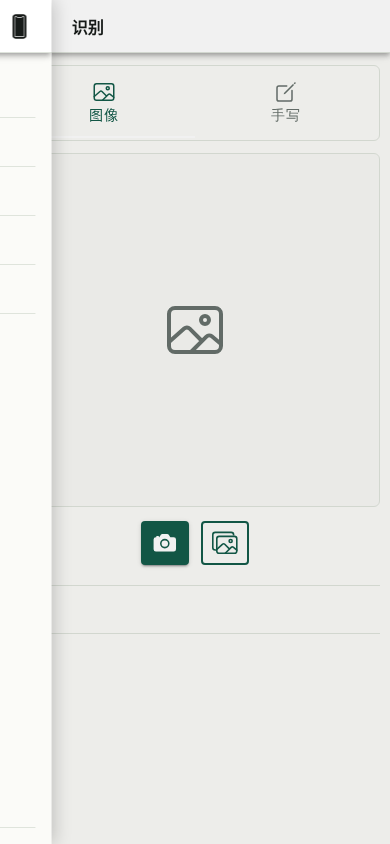
\includegraphics[width=\textwidth,height=0.36\textheight,keepaspectratio]{30-mobile-locale-zh-cn.png}
    \caption{the mobile interface with Simplified Chinese selected}
    \label{fig:locale-zh-cn}
  \end{subfigure}
  \hfill
  \begin{subfigure}[t]{0.31\textwidth}
    \centering
    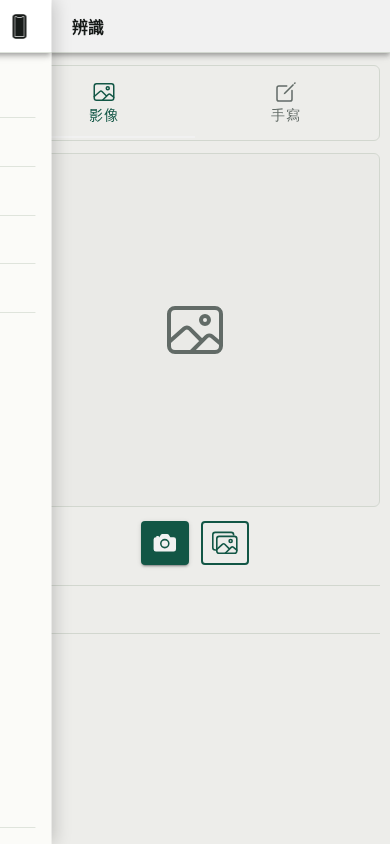
\includegraphics[width=\textwidth,height=0.36\textheight,keepaspectratio]{31-mobile-locale-zh-tw.png}
    \caption{the mobile interface with Traditional Chinese selected}
    \label{fig:locale-zh-tw}
  \end{subfigure}
\end{figure}

\begin{figure}[H]
  \centering
  \begin{subfigure}[t]{0.31\textwidth}
    \centering
    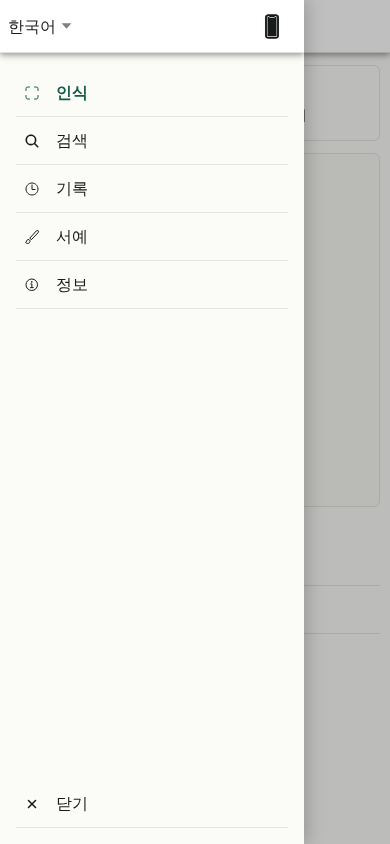
\includegraphics[width=\textwidth,height=0.36\textheight,keepaspectratio]{32-mobile-locale-ko-kr.png}
    \caption{the mobile interface with Korean selected}
    \label{fig:locale-ko-kr}
  \end{subfigure}
  \hfill
  \begin{subfigure}[t]{0.31\textwidth}
    \centering
    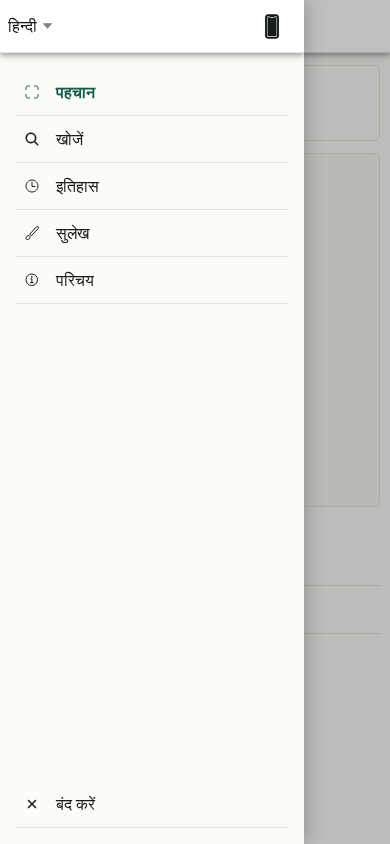
\includegraphics[width=\textwidth,height=0.36\textheight,keepaspectratio]{33-mobile-locale-hi-in.png}
    \caption{the mobile interface with Hindi selected}
    \label{fig:locale-hi-in}
  \end{subfigure}
  \hfill
  \begin{subfigure}[t]{0.31\textwidth}
    \centering
    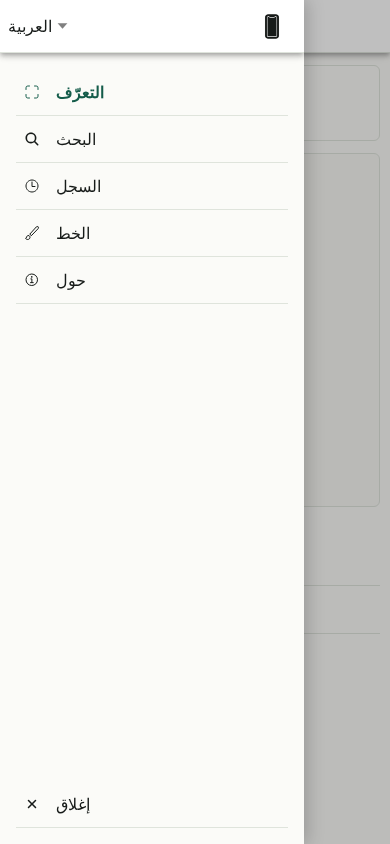
\includegraphics[width=\textwidth,height=0.36\textheight,keepaspectratio]{34-mobile-locale-ar-sa.png}
    \caption{the mobile interface with Arabic selected}
    \label{fig:locale-ar-sa}
  \end{subfigure}
\end{figure}

\begin{figure}[H]
  \centering
  \begin{subfigure}[t]{0.31\textwidth}
    \centering
    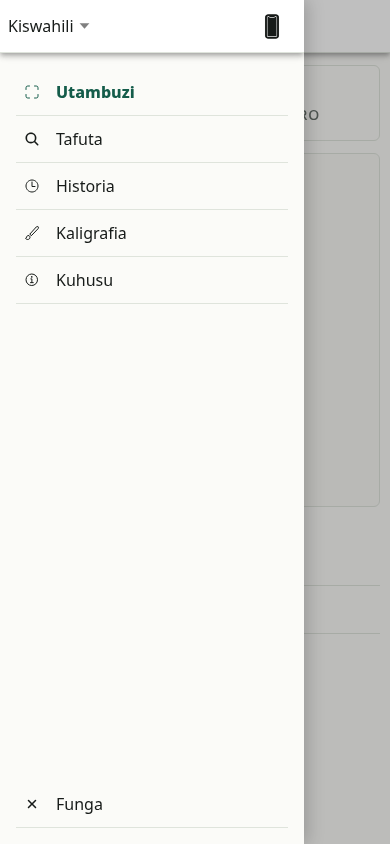
\includegraphics[width=\textwidth,height=0.36\textheight,keepaspectratio]{35-mobile-locale-sw-ke.png}
    \caption{the mobile interface with Kiswahili selected}
    \label{fig:locale-sw-ke}
  \end{subfigure}
  \hfill
  \begin{subfigure}[t]{0.31\textwidth}
    \centering
    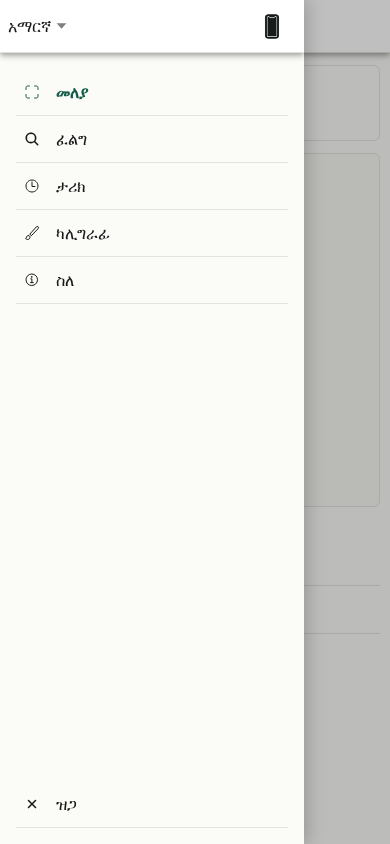
\includegraphics[width=\textwidth,height=0.36\textheight,keepaspectratio]{36-mobile-locale-am-et.png}
    \caption{the mobile interface with Amharic selected}
    \label{fig:locale-am-et}
  \end{subfigure}
  \hfill
  \begin{subfigure}[t]{0.31\textwidth}
    \centering
    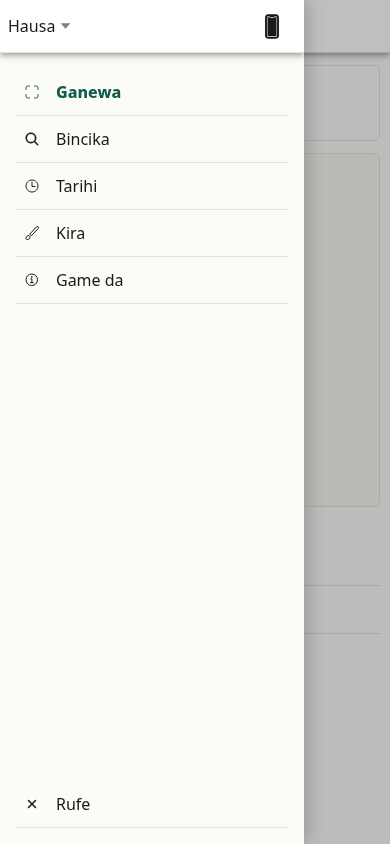
\includegraphics[width=\textwidth,height=0.36\textheight,keepaspectratio]{37-mobile-locale-ha-ng.png}
    \caption{the mobile interface with Hausa selected}
    \label{fig:locale-ha-ng}
  \end{subfigure}
\end{figure}

\begin{figure}[H]
  \centering
  \begin{subfigure}[t]{0.31\textwidth}
    \centering
    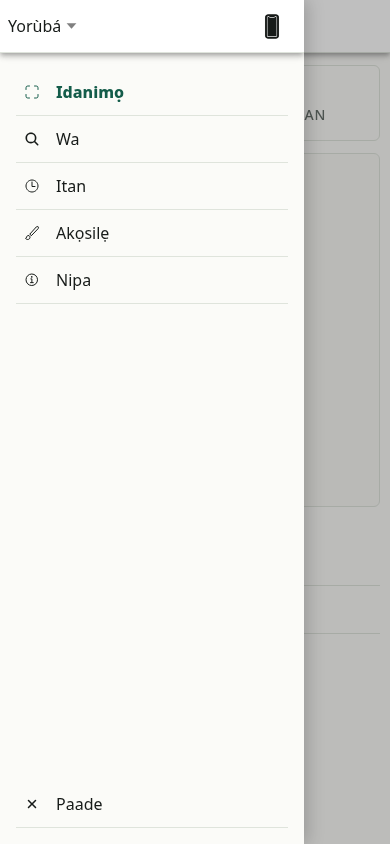
\includegraphics[width=\textwidth,height=0.36\textheight,keepaspectratio]{38-mobile-locale-yo-ng.png}
    \caption{the mobile interface with Yorùbá selected}
    \label{fig:locale-yo-ng}
  \end{subfigure}
  \hfill
  \begin{subfigure}[t]{0.31\textwidth}
    \centering
    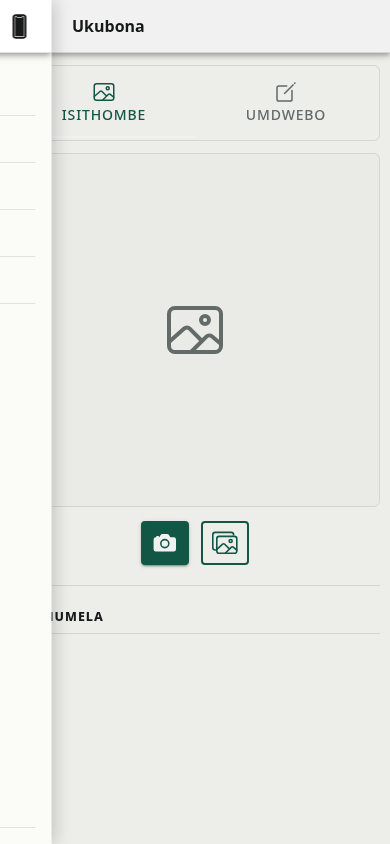
\includegraphics[width=\textwidth,height=0.36\textheight,keepaspectratio]{39-mobile-locale-zu-za.png}
    \caption{the mobile interface with isiZulu selected}
    \label{fig:locale-zu-za}
  \end{subfigure}
\end{figure}

\newpage
\thispagestyle{empty}
\vspace*{\fill}
\begin{center}
  {\color{accent}\rule{0.82\textwidth}{2pt}\par}
  \vspace{1.4cm}
  {\Huge\bfseries KanjiMe Admin\par}
  \vspace{0.8cm}
  {\LARGE Administration Panel\par}
  \vspace{1.4cm}
  {\color{accent}\rule{0.82\textwidth}{2pt}\par}
\end{center}
\vspace*{\fill}
\newpage

\newpage
\section{Administration Panel}

\subsection{Authentication}

The administration panel restricts access to authorised Google accounts.
Authentication protects version configuration and error-report data from the
public interface.

The initial form contains a single Google sign-in action, as shown in
Figure~\ref{fig:admin-login}. No account-registration or credential-recovery
controls appear in this view. During authentication, the state in
Figure~\ref{fig:admin-signing-in} replaces the normal action label. A failed
session displays the message in Figure~\ref{fig:admin-authentication-error}.

\desktopcapture{12-admin-login.png}
  {the administrator login screen before authentication}
  {fig:admin-login}

\desktopcapture{69-admin-auth-signing-in.png}
  {the administrator authentication-in-progress state}
  {fig:admin-signing-in}

\desktopcapture{70-admin-auth-error.png}
  {the administrator authentication error state}
  {fig:admin-authentication-error}

\subsection{Dashboard}

The Dashboard is the first protected view after authentication. It summarises
the administration area and provides access to the technical-support sections.

Dashboard data is loaded before the summary becomes available. The completed
view appears in Figure~\ref{fig:admin-dashboard}. The loading state in
Figure~\ref{fig:admin-dashboard-loading} and failure state in
Figure~\ref{fig:admin-dashboard-error} keep the administrator informed when
that data is not ready.

\desktopcapture{13-admin-dashboard.png}
  {Authenticated administration dashboard}
  {fig:admin-dashboard}

\desktopcapture{71-admin-dashboard-loading.png}
  {Dashboard loading state}
  {fig:admin-dashboard-loading}

\desktopcapture{73-admin-dashboard-error.png}
  {Dashboard error state}
  {fig:admin-dashboard-error}

\subsection{Version Configuration}

Version Configuration stores the release information consumed by the mobile
application. The protected view separates the current configuration from the
form used to change it.

The configuration overview appears in
Figure~\ref{fig:admin-version-configuration}. Editing exposes the configurable
fields in Figure~\ref{fig:admin-version-edit}. Validation prevents malformed
values from being submitted, as shown in
Figure~\ref{fig:admin-version-validation-error}.

\desktopcapture{14-admin-versions.png}
  {Authenticated version-configuration section}
  {fig:admin-version-configuration}

\desktopcapture{76-admin-versions-edit.png}
  {Version-configuration edit state}
  {fig:admin-version-edit}

\desktopcapture{77-admin-versions-validation-error.png}
  {Version validation-error state}
  {fig:admin-version-validation-error}

\subsection{Error Reports}

Error Reports presents unexpected runtime failures reported by the mobile
application. Each entry can be reviewed as a technical-support case without
mixing report management with version configuration.

The report list appears in Figure~\ref{fig:admin-error-reports}. Status filters
restrict the list to OPEN, IN PROGRESS, RESOLVED, CLOSED, or DISCARDED cases.
An empty state distinguishes a valid query with no matching reports from a
loading failure. These variants appear in
Figures~\ref{fig:admin-error-reports-empty},
\ref{fig:admin-error-reports-open}, \ref{fig:admin-error-reports-in-progress},
\ref{fig:admin-error-reports-resolved}, \ref{fig:admin-error-reports-closed},
and \ref{fig:admin-error-reports-discarded}.

\desktopcapture{15-admin-errors.png}
  {Authenticated error-report list}
  {fig:admin-error-reports}

\desktopcapture{79-admin-errors-empty.png}
  {Empty error-report list}
  {fig:admin-error-reports-empty}

\desktopcapture{80-admin-errors-filter-open.png}
  {Error-report list filtered by OPEN}
  {fig:admin-error-reports-open}

\desktopcapture{81-admin-errors-filter-in-progress.png}
  {Error-report list filtered by IN PROGRESS}
  {fig:admin-error-reports-in-progress}

\desktopcapture{82-admin-errors-filter-resolved.png}
  {Error-report list filtered by RESOLVED}
  {fig:admin-error-reports-resolved}

\desktopcapture{83-admin-errors-filter-closed.png}
  {Error-report list filtered by CLOSED}
  {fig:admin-error-reports-closed}

\desktopcapture{84-admin-errors-filter-discarded.png}
  {Error-report list filtered by DISCARDED}
  {fig:admin-error-reports-discarded}

\subsection{Error Detail}

Error Detail presents the information attached to one selected report. The view
keeps the report context and its current support status together.

The main detail content appears in Figure~\ref{fig:admin-error-detail}. A recent
actions area records the report activity available to the administrator, as
shown in Figure~\ref{fig:admin-error-detail-actions}.

\desktopcapture{16-admin-error-detail.png}
  {Authenticated error-detail view}
  {fig:admin-error-detail}

\desktopcapture{88-admin-error-detail-actions.png}
  {Error-detail recent-actions area}
  {fig:admin-error-detail-actions}

\newpage
\appendix
\section{Special States}

\subsection{Startup capture}

Startup prepares the local services required by the mobile application. Once
initialisation completes, the primary Recognition route becomes active.

The resulting view opens Recognition in empty Image mode, as shown in
Figure~\ref{fig:startup-recognition}. The camera and image-selection controls
are ready for input.

\mobilecapture{17-mobile-startup-loading.png}
  {the captured startup file, which visibly matches the initial Recognition state}
  {fig:startup-recognition}

\subsection{Update notice}

KanjiMe checks the configured release information and compares it with the
installed version. The normal study workflow remains visible while an available
update is announced.

When a newer release is detected, the toast in Figure~\ref{fig:update-toast}
informs the user without replacing the current view.

\mobilecapture{50-mobile-update-toast.png}
  {Application update toast}
  {fig:update-toast}

\subsection{Global error message}

Unexpected runtime failures are converted into a controlled user-facing state.
The message avoids implementation details and confirms that the requested
operation could not be completed.

The global alert appears in Figure~\ref{fig:global-error-dialog}. Errors tied to
a specific task remain within that task, as shown by the camera error in
Figure~\ref{fig:recognition-camera-error} and the lookup error in
Figure~\ref{fig:lookup-error}.

\mobilecapture{49-mobile-global-error-alert.png}
  {Global controlled-error alert}
  {fig:global-error-dialog}

\end{document}
